%!TEX root = ../deco_star.tex

%-------------------------------------------------------------------------

\section{Models}
\label{sec:models}

In the context of computer graphics, generation techniques are usually differentiated into procedural and data-driven approaches. This understanding applies equally to the generation of geometry, animations and texture, for example. Procedural techniques describe the visual output by evaluating an algorithm, while data-driven approaches rely on existing data, such as photographs. However, through the continuous development of both fields, approaches started to blend and the advantages of both approaches are brought together. 

For this goal, this survey focuses on procedural models as a basis, but it also integrates and highlights promising or desirable characteristics of suitable data-driven techniques.

\subsection{Procedural}
\label{subsec:models_procedural}

\citeauthor*{ebert_2003_tmp}~\cite{ebert_2003_tmp} describe procedural techniques as algorithms and mathematical functions that synthesize a model or an effect. Solely equation-based representations are considered the ``purest'' form of procedural modeling~\cite{smelik_2014_aso}. This approach gained immediate importance in the early days of computer graphics. Analytical forms are able to reproduce many natural phenomena -such as wood, stone, water, smoke and plants- with only some lines of code in the range of kilobytes, hence being memory efficient. The main appeals of such procedural representation include its compactness in combination with being continuous, scalable and unbound to a specific resolution. While procedural generation techniques have been a constant basis for generating content for games, its characteristics of memory efficiency and unlimited resolution are more important than ever with the rise of virtual reality, for example.

The compactness and efficiency of a procedural model also enable parameterization, resulting in the model being responsive and flexible. Parameters usually represent certain visual characteristics and their amplification. Parameterization brings the crucial benefit that, for example, textures remain editable throughout the entire visual effect production pipeline.

However, the effectiveness of traditional parameterization in helping an artist fulfill design goals is debatable. \citeauthor*{ebert_2003_tmp}~\cite{ebert_2003_tmp} argue that parameterization brings the benefit of a few parameters controlling large amounts of details. At the same time, this is potentially problematic for the realization of specific designs because these often require full individual control of all visual elements. Additionally, parameters are often non-intuitive due to representing overly abstract characteristics of the underlying functions and having overlapping effects~\cite{bourque_2004_ptm,lagae_2010_pis,gilet_2010_ias,benes_2011_gpm,lasram_2012_ssf,lasram_2012_ptp}.

In addition to the disadvantage in the control of a procedural representation, the creation of the representation itself, the procedural model, requires considerable effort - even though it is only a one-time investment. For the appearance of a model, the focus usually lies on a more generic design, like a texture class. For procedural textures specifically, handling antialiasing efficiently can also be challenging. For a valuable and in-detail survey of function-based design principles of procedural models with focus on textures, the interested reader is referred to \citeauthor*{ebert_2003_tmp}~\cite{ebert_2003_tmp}. Procedural models are not limited to purely function-based designs. For example, the pioneering work of \citeauthor*{Prusinkiewicz_2012_TAB}~\cite{Prusinkiewicz_2012_TAB} applies the grammar-based L-system to algorithmically model plant growth, an approach extensively investigated by the computer graphics community and considered as procedural.

The classifications of core mechanisms for procedural generation of \citeauthor*{hendrikx_2013_pcg}~\cite{hendrikx_2013_pcg} in the context of games and the categorization of \citeauthor*{smelik_2014_aso}~\cite{smelik_2014_aso} for virtual worlds are equally appropriate in the context of creative pattern generation. In the following we briefly discuss core mechanisms in the context of creative pattern generation, based on the previously mentioned taxonomies (\cite{hendrikx_2013_pcg}, \cite{smelik_2014_aso}).

\paragraph*{Stochastic Models} generate models by using random values. They can either be used in their original form as procedural model or as a noise basis function. Visual features can be added by combining multiple layers of the noise in different resolutions. Typical noise functions are lattice value noise, lattice gradient noise (\eg~Perlin noise \cite{perlin_1985_ais}), sparse convolution noise and spectral noise~\cite{ebert_2003_tmp,lagae_2010_sap}. 
% These ``pure'' procedural programs also have the advantage of being well suited for optimization, such as parallelization, because they can be randomly evaluated in constant time~\cite{lagae_2010_sap}. 
In the context of creative pattern generation, stochastic models build a basis for many designs but their design spectrum and controllability are limited.

\paragraph*{Function-based Models} extend the class of stochastic models by layering and combining a variety of functions to form a visually complex pattern. Typical building blocks are periodic, spline, step, clamp and conditional functions~\cite{ebert_2003_tmp} and are the basis for regular patterns designs. 

\paragraph*{Rule-based Models} are part of individual, and often quite complex, generation systems that can be context-dependent and/or design-specific. Rule-based models are programs that relate to and partition the space to fill and follow propagation rules. The algorithmic core often handles proxy shapes, while for the result graphical elements, such as vector graphics, are mapped to the proxies. Rule-based procedural models are suitable for creative pattern generation and novel control mechanisms because their iterative generation logic is open and flexible~\cite{wong_1998_cgf, mech_2012_tdf}. They can implement any designs and include any elements. Moreover, within a suitable pipeline, they can potentially take global constraints into consideration and build structural hierarchies.

\paragraph*{Grammar-based Models}
% Grammar-based models are also considered ``purely'' procedural~\cite{smelik_2014_aso}. 
form grammatically-correct sentences from individual words, based on a system of rules, and they are related to rule-based models in that the rules are using grammars or rewriting systems. 
% Originally introduced in theoretical linguistics by Noam Chomsky in the late 1950s, grammars are applied in computer graphics to generate objects such as plants from elements encoded as letters or words~\cite{hendrikx_2013_pcg}. 
Prominent techniques are L-systems and shape grammars. An emerging subgroup of grammar-based models includes \textit{probabilistic} inference into the derivation of correct sentences from a grammar. In recent years, there have been a variety of successful grammar-based approaches for certain aspects of creative pattern generation~\cite{benes_2011_gpm,talton_2011_mpm,ritchie_2015_cpm}. However, grammars are difficult to set up and to design~\cite{stava_2010_ipm}. Because the execution process is inherently hierarchical, grammar systems have difficulty in supporting creative control from a global to local scale.

% \textit{Simulation Models:} Simulation models are based on techniques that approximate complex phenomena for which an analytical solution is unmanageable or unavailable. \citeauthor*{hendrikx_2013_pcg}~\cite{hendrikx_2013_pcg} further group simulation techniques into cellular automata, vector and tensor fields, and agent-based simulations. 

% In the context of creative pattern generation, simulation models are not prominent, with the exception of vector and tensor fields~\cite{ijiri_2008_aeb,yuanyuan_2011_gso,saputra_2017_ffo}. For simulation models usually interactive performance is a challenge, as well as the control on an element level. However, the potential to create a layout within a space and adapt to the characteristics of that space within a simulation system as well as the possible design variability call for further investigation.

\paragraph*{Artificial Intelligence Models} represent approaches that go beyond the direct execution of specific rules. For example, they automatically optimize results based on fitness or error functions, or they apply planning steps. \citeauthor*{hendrikx_2013_pcg}~\cite{hendrikx_2013_pcg} group this class into genetic algorithms, neural networks and constraint satisfaction and planning. In recent years, machine learning has been introduced into procedural content generation with the same impact as in all other computer science fields~\cite{summerville_2017_pcg}. The potential of machine learning techniques in regard to creative pattern generation and their control mechanisms seems almost limitless.
% and is further discussed as outlook in \Cref{subsec:analysis_outlook_mixed_initiative_interfaces}.



\subsection[Data-Driven]{Data-Driven Models}
\label{subsec:design_models_datadriven}

In contrast to procedural techniques, data-driven methods can be used in two ways in the context of creative pattern generation. First, they describe the processing of input pixel data, such as a photograph. Second, they refer to the output of a method, which is again pixel data. Data-driven models traditionally do not include underlying design models, as procedural representations do. Consequently, data-driven approaches are flexible in terms of possible designs and can achieve photorealism by processing real photographs.

At the same time, photographs bring the disadvantage of potentially including visual features, such as illumination effects that are unwanted and difficult to remove. Moreover, further down a production pipeline, pixel data is usually not editable anymore. Working with data such as high-resolution images leads to high memory requirements, and without additional algorithms, data is fixed to its given resolution and scale.

% Does this section really fit here?
Addressing the issue of resolution example-based synthesis is a well-established field of research and aims to create infinite amounts of pixel data based on a given exemplar. The pyramid-based texture synthesis of \citeauthor*{heeger_1995_pbt}~\cite{heeger_1995_pbt} is an early famous example.~\citeauthor*{wei_2009_seb}~\cite{wei_2009_seb}, as well as~\citeauthor*{barnes_2017_aso}~\cite{barnes_2017_aso} present comprehensive summaries of such example-based texture synthesis techniques, discussing statistical feature matching, neighborhood matching, patch-based and optimization methods. Overall, example-based methods for texture synthesis have achieved similar results in data size, random accessibility and editing and resolution options as procedural textures - but only within specialized contexts and not in an unified manner. Procedural textures offer these capabilities as inherent and combined characteristics.

Data-driven models are numerous and diverse because they can use and produce any input and output data without an underlying procedural model. In the following survey of the state of the art for creative pattern generation, we include various data-driven techniques, however an overall classification is not the focus of this work. Relevant techniques include the tiling and distribution of elements and drawing and brush mechanisms.

% For a review of models that output ornamental patterns, we focus on the output of the models and not on their underlying generation principles in order to come to a summarization.


\subsection{Specific Pattern Designs}
\label{subsec:specific_pattern_designs}

In this section we review models that output specific pattern designs, exemplary for creative pattern generation. The references in this section summarize work that solely focus on the output and hardly offer any control mechanisms or support a creative creation process. Work that produces similar aesthetics but also offer control mechanisms (\eg~\cite{wong_1998_cgf,yu_2012_ans,zehnder_2016_dso}), are reviewed in~\Cref{sec:analysis}~\nameref{sec:analysis}.

%  Celtic designs were, for example, successfully computed by~\citeauthor*{kaplan_2003_cgc}~\cite{kaplan_2003_cgc} and~\citeauthor*{doyle_2013_ccc}~\cite{doyle_2013_ccc}.

Work on the generation of pattern designs is spread over various research communities~\cite{whitehead_2010_tpd}. For the development of models \citeauthor*{whitehead_2010_tpd}~\cite{whitehead_2010_tpd} differentiates between two motivations in the context of generating models for ornamentation in games. First, the author identifies the goal to reproduce existing patterns such as Islamic and Celtic designs. Such work is mainly found in the communities of mathematics and computer science. Second, \citeauthor*{whitehead_2010_tpd} identifies the goal of generating novel pattern designs, which is held mainly by algorithmic computer artists. Such designs are usually not executed in an academic context and, beyond the presentation of the results, are unfortunately not well documented. Only a few exceptions, such as the work of \citeauthor*{takayama_2016_med}~\cite{takayama_2016_med} in regard to 3D-printed ornate shapes or \citeauthor*{alvarez_2019_ido}~\cite{alvarez_2019_ido} for randomized abstract texture designs give some information about their underlying algorithms. However, due to the overall missing comparable documentations we do not further include computer artists' work.

For what \citeauthor*{whitehead_2010_tpd}~\cite{whitehead_2010_tpd} calls mathematic/scientific ornamentation in the context of games, the author 
% In the following, we summarize and extend the analysis of~\citeauthor*{whitehead_2010_tpd}~\cite{whitehead_2010_tpd} regarding what he calls mathematic/scientific ornamentation. \citeauthor*{whitehead_2010_tpd}~\cite{whitehead_2010_tpd}'s survey does not necessarily follow ornamental design rules, all examples constitute at least a subpart of an ornament - for example, the background fillings. These publications focus on the analysis of a pattern and the development of a generative model for a specific pattern type rather than its controllability. Hence, we do not include these in the taxonomy of control mechanisms.
% 
% Rigid design rules enable formal models and~\citeauthor*{whitehead_2010_tpd}~\cite{whitehead_2010_tpd} 
describes tiling and symmetry as the most relevant constituting rules. In combination with interlacing parts of the pattern while repeating and tiling elements, these principles are able to systematically describe Islamic~\cite{ostromoukhov_1998_mtc} and Celtic~\cite{cromwell_1993_ckm} patterns, towards the traditional designs given in \Cref{fig:islamic_celtic_ornament}.

%LG: Take this figure out?
\begin{figure}
\centering
    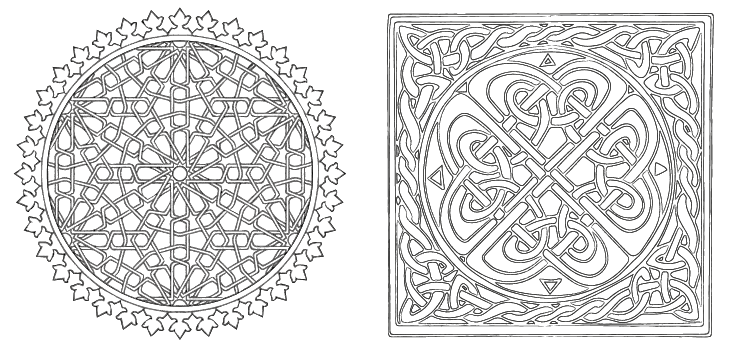
\includegraphics[width=0.9\columnwidth]{figures/islamic_celtic_ornament_01.png}
    \caption[Islamic and Celtic pattern designs]{Examples of traditional Islamic (left) and Celtic pattern designs, showing the complexity of possible pattern designs. Image sources: [12, 13].}
\label{fig:islamic_celtic_ornament}
\end{figure}

The seminal work of \citeauthor*{kaplan_2004_isp}~\cite{kaplan_2004_isp} presents an algorithmic representation of Islamic star patterns, a topic of ongoing interest~\cite{khamjane_2018_giq}. Readers further interested in this line of work are referred to the extensive investigation of~\citeauthor*{kaplan_2002_cgg}~\cite{kaplan_2002_cgg}. \citeauthor*{etemad_2008_apf}~\cite{etemad_2008_apf} and~\citeauthor*{hamekasi_2012_dpf}~\cite{hamekasi_2012_dpf} also focus on Islamic flower patterns. Celtic designs were, for example, also successfully computed by~\citeauthor*{kaplan_2003_cgc} and~\cite{doyle_2013_ccc}.

In addition to Islamic and Celtic designs, a variety of other pattern designs have been algorithmically formalized, such as Gothic window tracery~\cite{havemann_2004_gpd}, M. C. Escher patterns~\cite{dunham_1981_crh,kaplan_2004_isp}, woodwork~\cite{gulati_2010_acp,gulati_2012_acp}, optical illusions~\cite{chi_2014_ois}, mazes~\cite{pedersen_2006_ola} and tile-based patterns~\cite{ouyang_2015_cat, gdawiec_2017_pga}.


% %-------------------------------------------------------------------------

\subsection{Summary}
\label{subsec:models_summary}

To produce designs that include not only repetitive structures but also visual hierarchies and highlights for example, most procedural models in their "pure" form are too limited in their design variability. Data-driven models are more flexible in both their design space and creative control mechanisms. However, data-driven models are tedious, not suitable for automatically executing certain design rules, and they are limited in the data they use. The following review of the state of the art gives a detailed comparison of the capabilities for creative pattern generation.